\label{chap:ExpRes}
Based on sections \ref{sec:neuralNet} and \ref{sec:imgClass}, in this chapter, we will discuss further about the experimental results, particularly of the image classification, distance estimation and object detection problems.

\section{Image Classification}
\label{sec:imgClasEval}
\subsection{Problem Review}
Remember that the problem we are referring in this section is the image classification of images belonging to 12 categories. We have the following details:
\begin{enumerate}
	\item 12 classes: \tit{"apple", "pen", "book", "monitor", "mouse", "wallet", "keyboard", "banana", "key", "mug", "pear", "orange"}.
	\item 1200 images for each class.
	\item Divide the whole dataset into 30\% test set (4320 images), 56\% training set (8064 images) and 14\% validation set (2016 images).
	\item Experiments with multiple options: 
	\begin{itemize}
		\item with/without fine-tuning
		\item with/without image preprocessing
		\item with/without data augmentation
		\item multiple based models (Resnet50, VGG16, Xception)
		\item multiple configuration for fully-connected layer (number of hidden layer, etc.)
	\end{itemize} 
	\item Note that after convolutional block, we flatten the feature tensor to become a 1D feature vector. In addition, our number of classes is fixed to 12. Hence we only denote the hidden layers in the fully-connected part. For example, resnet\_512 is the model uses convolutional blocks of Resnet50 and has fully-connected part as: flatten - 512 - 12. 
	\item Training is done entirely by an Azure NV12 instance which has a GPU Nvidia M60 16GB. Using Resnet50, each epoch takes us $\approx 90$ seconds. We have to train the classifier system $\approx 26$ epochs ($\approx 45 minutes$) to achieve $ > 93\%$ top-1 accuracy.
\end{enumerate}

\subsection{Transfer Learning Result}
\label{sec:transLearnEval}
%\subsection{Results and Observations}
As discussed in subsection \ref{sec:transferLearning}, we can freely design the fully-connected part. After multiple experiments, I found the following interesting observations:
\begin{enumerate}
	\item Bigger fully-connected parts only helps to train the system in fewer epochs. This is reasonable because more complex models has more capacity. However, the trade-off is that we have a bigger model size and it is slower at test time. (figure \ref{fig:compareResnetNoFT})
	\item Fine-tuning the final convolutional block improves the accuracy about 2-3\% (figure \ref{fig:accResnet128NoFT} vs figure \ref{fig:accResnet128})
	\item Image augmentation do not help much in my situation (\ref{fig:compareResnet}). We can see that models with augmented data have better performance in the beginning. However at the end, they are all rougly the same.
	\item As expected, zero-centering and normalization improves a bit the training accuracy (i.e. faster training) but does not improve significantly the validation accuracy. (figures \ref{fig:resnet512StMean}, \ref{fig:accResnet512}, \ref{fig:resnet512StMeanScale}, \ref{fig:accResnet512dup}) I think the reason that it does not improve validation accuracy significantly is the difficulty of our dataset.
	\item Resnet50 is the best base model among VGG16, Xception and Resnet50 (more details are shown in figure \ref{fig:compareModels}). A more carefully fine-tuned version of resnet\_512 model can reach to 94.2\% on validation accuracy.
	\item Accuracy on test set is $\approx$ 93.5\% - 93.7\%. Prediction details can be found in table \ref{table:1}. 
	\item Remark that our dataset is difficult because:
	\begin{itemize}
		\item one image can contain objects of several classes belonging to the 12 categories
		\item the ground truth object does not necessarily appear largely at the center of the image
	\end{itemize}
	Figure \ref{fig:testFail1} and \ref{fig:testFail2} illustrate 2 examples where the system predicts wrongly.
\end{enumerate}
	

\begin{figure}[tb]
	\centering
	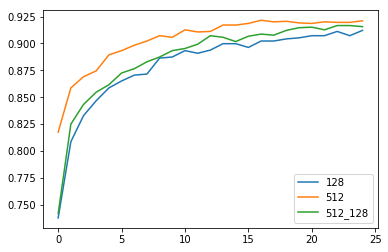
\includegraphics[width=0.6\hsize]{./figures/compareResnetNoFT}
	\caption{Comparison of Resnet models with different fully-connected parts: 128, 512, 512\_128. We can see that bigger model (512) has more capacity and reach the baseline 90\% faster. Multiple layers (512\_128) on the other hand performs worse than one big layer (512).}
	\label{fig:compareResnetNoFT}
\end{figure}

\begin{figure}[!ht]
	\centering
	\begin{minipage}[t]{0.45\linewidth}
		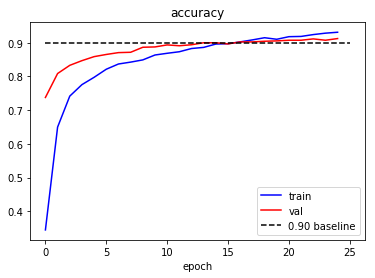
\includegraphics[scale=0.5]{./figures/accResnet128NoFT}
		\caption{resnet\_128 without finetuning: validation accuracy reaches to  $\approx$ 91.6\%}
		\label{fig:accResnet128NoFT}
	\end{minipage}
	\centering
	\begin{minipage}[t]{0.45\linewidth}
		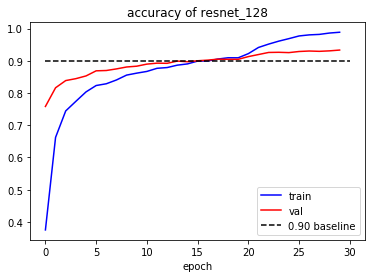
\includegraphics[scale=0.5]{./figures/accResnet128}
		\caption{resnet\_128 fine-tuned around epoch 18: validation accuracy reaches to $\approx$ 93.3\%}
		\label{fig:accResnet128}
	\end{minipage}
\end{figure}


\begin{figure}[tb]
	\centering
	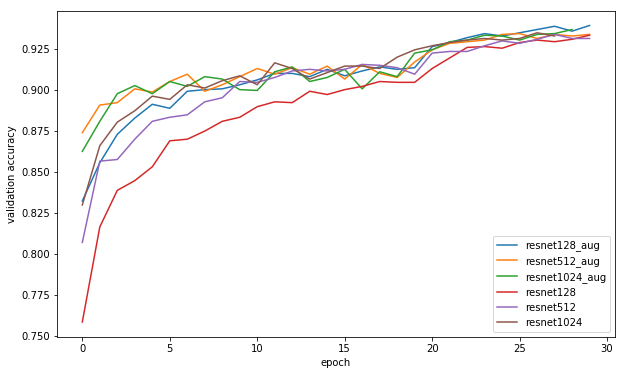
\includegraphics[width=0.8\hsize]{./figures/compareResnet}
	\caption{Comparison of Resnet models with different fully-connected parts: 128, 512, 1024 and with/without data augmentation. We can see that augmentation data does not help much in the end. In the beginning, the accuracy when applying data augmentation is higher because the system is trained on the augmented images (i.e. more training data). Note that all models jumped up around epoch 20 when I applied fine-tuning.}
	\label{fig:compareResnet}
\end{figure}


\begin{figure}[!ht]
	\centering
	\begin{minipage}[t]{0.45\linewidth}
		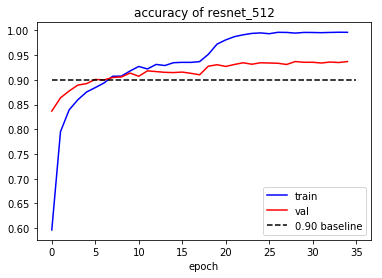
\includegraphics[scale=0.5]{./figures/resnet512StMean}
		\caption{resnet\_512 with mean of training data subtracted. Train accuracy is a bit higher at the beginning.}
		\label{fig:resnet512StMean}
	\end{minipage}
	\centering
	\begin{minipage}[t]{0.45\linewidth}
		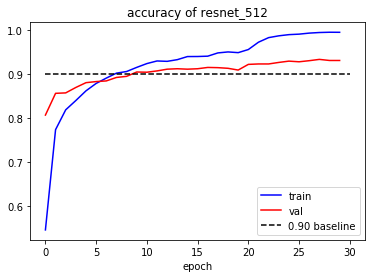
\includegraphics[scale=0.5]{./figures/accResnet512}
		\caption{resnet\_512 with no preprocessing. Both two versions reach $\approx 93.7\%$ validation accuracy at the end.}
		\label{fig:accResnet512}
	\end{minipage}
\end{figure}

\begin{figure}[!ht]
	\centering
	\begin{minipage}[t]{0.45\linewidth}
		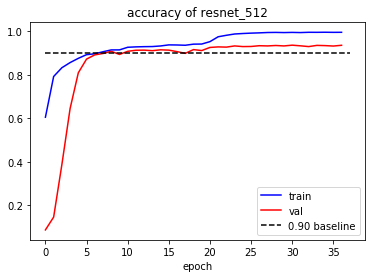
\includegraphics[scale=0.5]{./figures/resnet512StMeanScale}
		\caption{resnet\_512 with both mean of training data subtracted and scaled by dividing to 255. Training is a bit faster but validation accuracy is improving more slowly.}
		\label{fig:resnet512StMeanScale}
	\end{minipage}
	\centering
	\begin{minipage}[t]{0.45\linewidth}
		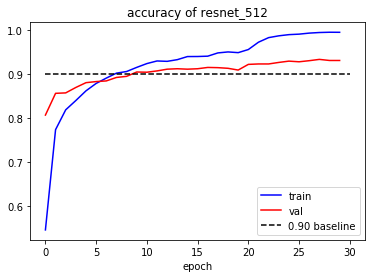
\includegraphics[scale=0.5]{./figures/accResnet512}
		\caption{resnet\_512 with no preprocessing. Both two versions reach $\approx 93.7\%$ validation accuracy at the end.}
		\label{fig:accResnet512dup}
	\end{minipage}
\end{figure}


\begin{figure}[tb]
	\centering
	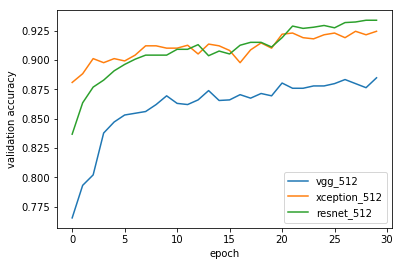
\includegraphics[width=0.7\hsize]{./figures/compareModels}
	\caption{Comparison accross models: VGG16, Resnet50, Xception with the same fully-connected layer (512). We see clearly the model capacity affects the result: VGG16 can not reach base-line 90\% while advanced models like Resnet50 and Xception easily get over 92\%. More precisely, Resnet50 is the best with accuracy greater than $93\%$) and Xception's accuracy is around $92.5\%$.}
	\label{fig:compareModels}
\end{figure}

\begin{figure}[tb]
	\centering
	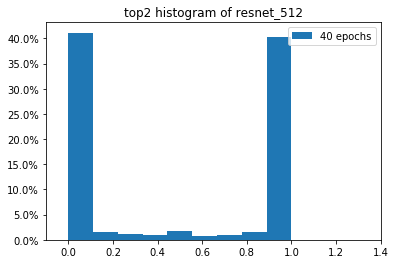
\includegraphics[width=0.6\hsize]{./figures/top2Histo}
	\caption{Histogram of Top 2 predictions probability on test set after training. As expected the trained model is quite sure about its predictions (mostly in $>0.9$ for the maximal probability and $<0.1$ for the second maximal probability). Some samples in the middle represents well the case it is confused due to the difficulty of the dataset.}
	\label{fig:top2Histo}
\end{figure}

\begin{table}[h!]
	\centering
\scriptsize		
	\begin{tabular}{ |c|c|c|c|c|c|c|c|c|c|c|c|c| } 
		\hline
 class &  apple &  pen &  book &  monitor &  mouse &  wallet &  keyboard &  banana &  key &  mug &  pear &  orange \\
 \hline
 apple &  \tbf{0.83} &  0.00 &  0.01 &  0.00 &  0.01 &  0.00 &  0.00 &  0.03 &  0.00 &  0.00 &  0.05 &  0.07 \\
 \hline
 pen &  0.00 &  \tbf{0.96} &  0.00 &  0.00 &  0.01 &  0.01 &  0.00 &  0.00 &  0.01 &  0.00 &  0.00 &  0.00 \\
 \hline
 book &  0.00 &  0.01 &  \tbf{0.96} &  0.01 &  0.00 &  0.02 &  0.00 &  0.00 &  0.00 &  0.00 &  0.00 &  0.00 \\
 \hline
 monitor &  0.00 &  0.01 &  0.01 &  \tbf{0.94} &  0.02 &  0.01 &  0.01 &  0.00 &  0.00 &  0.00 &  0.00 &  0.00 \\
 \hline
 mouse &  0.01 &  0.00 &  0.00 &  0.03 &  \tbf{0.88} &  0.01 &  0.04 &  0.00 &  0.01 &  0.01 &  0.01 &  0.00 \\
 \hline
 wallet &  0.00 &  0.00 &  0.01 &  0.01 &  0.00 &  \tbf{0.96} &  0.00 &  0.00 &  0.02 &  0.00 &  0.00 &  0.00 \\
 \hline
 keyboard &  0.00 &  0.00 &  0.00 &  0.04 &  0.02 &  0.00 &  \tbf{0.94} &  0.00 &  0.00 &  0.00 &  0.00 &  0.00 \\
 \hline
 banana &  0.02 &  0.00 &  0.00 &  0.00 &  0.00 &  0.00 &  0.00 &  \tbf{0.95} &  0.00 &  0.00 &  0.00 &  0.03 \\
 \hline
 key &  0.00 &  0.00 &  0.01 &  0.00 &  0.00 &  0.01 &  0.00 &  0.00 &  \tbf{0.97} &  0.00 &  0.00 &  0.00 \\
 \hline
 mug &  0.00 &  0.00 &  0.00 &  0.00 &  0.00 &  0.00 &  0.00 &  0.01 &  0.00 &  \tbf{0.99} &  0.00 &  0.00 \\
 \hline
 pear &  0.05 &  0.00 &  0.00 &  0.00 &  0.00 &  0.00 &  0.00 &  0.01 &  0.00 &  0.00 &  \tbf{0.91} &  0.02 \\
 \hline
 orange &  0.03 &  0.00 &  0.00 &  0.00 &  0.00 &  0.00 &  0.00 &  0.02 &  0.00 &  0.00 &  0.03 &  \tbf{0.92} \\
 \hline
	\end{tabular}
\caption{Prediction table: each row represents percentage of the system's predictions on the corresponding class. Consider the first row for example: for all images of ground truth \tit{apple}, the systems predicts correctly 83\%, 17\% wrong predictions false mostly to \tit{orange}, \tit{pear}. This is acceptable as noted previously that many fruit images contain objects of mixed classes.}
\label{table:1}
\end{table}

\begin{figure}[!ht]
	\centering
	\begin{minipage}[t]{0.45\linewidth}
		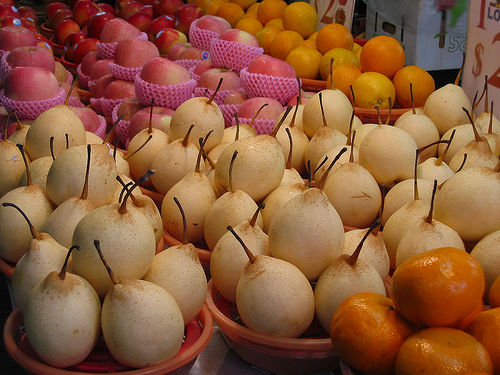
\includegraphics[scale=0.35]{./figures/testFail1}
		\caption{Model predicts \tit{orange} while ground truth is \tit{pear}. We can see that oranges appear in lower right corner and this type of pear is quite special.}
		\label{fig:testFail1}
	\end{minipage}
	\quad
	\begin{minipage}[t]{0.45\linewidth}
		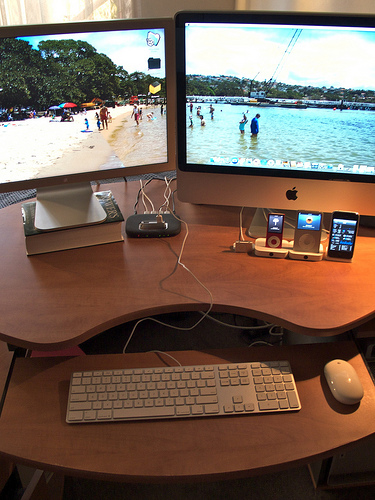
\includegraphics[scale=0.45]{./figures/testFail2}
		\caption{Model predicts \tit{monitor} while ground truth is \tit{keyboard}. We can see 2 bigs monitor in the upper of the image.}
		\label{fig:testFail2}
	\end{minipage}
\end{figure}

\section{Distance Estimation}
\label{sec:distEstimExp}
\subsection{Problem Review}
Distance Estimation is one of the most important task in Robot Localization and Mapping (or Simultaneous Localization and Mapping \cite{wiki:SLAM}). Given the camera's parameters and the size of the object, we can estimate the distance from the camera to the object. The theoretical notions are presented in \ref{sec:camModel}. In this section, we focus on setting up an experiment to verify those notions as well as to quantitatively estimate the order of magnitude of the error.

\subsection{Experiment and Result}
The experiment is setup with the Cozmo robot facing straight ahead a cube. The cube size is 4.4cm (i.e $w = h = 4.4cm$). Remember that all camera parameters are presented in subsection \ref{subsec:camInfo}. The cube is placed at ground truth distance $z \in \{10, 20, 30, 40, 50\}$ (centimeters). Figure \ref{fig:distEstim} illustrates this point. 

\begin{figure}[tb]
	\centering
	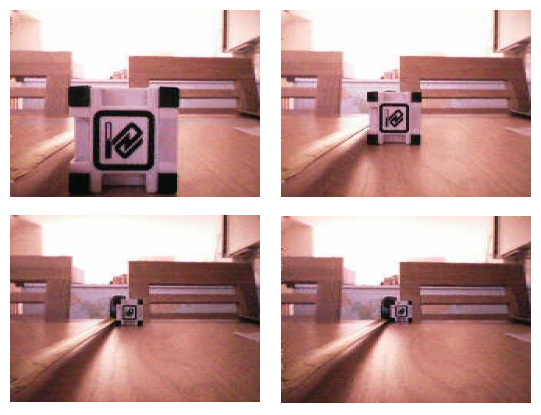
\includegraphics[width=0.6\hsize]{./figures/distEstim}
	\caption{Distance Estimation Experiment: a cube is placed in front of a Cozmo at distances $z = {10, 20, 40, 50}$ centimeters along the $z$ axis. We can see that there is no significant difference between $z = 40$ and $z = 50$ (centimeters). The size of the cube in the image are $w_i \approx {135, 70, 35, 28}$ (pixels) respectively.}
	\label{fig:distEstim}
\end{figure}

Explicitely, we will:
\begin{enumerate}
	\item compute $x_c, y_c, z$ from formula \ref{form:distEst} and \ref{form:centerIm}:
	\begin{align*}
	z = \frac{1}{2} (f_1 \frac{w}{w_i} + f_2 \frac{h}{h_i}) \hspace{0.5cm}
	x_c = \frac{1}{2}\frac{(u_1 + u_2 - 2  c_1)z}{f_1} \hspace{0.5cm} y_c = \frac{1}{2}\frac{(v_1 + v_2 - 2c_2)z}{f_2}
	\end{align*}
	\item compute distance $d$ and verify that $d \approx z$ ($z$ calculated above):
	$$d = \sqrt{x^2 + y^2 + z^2}$$
	\item estimate absolute error $\Delta z$ and relative error $\Delta z / z$ which is close to $\Delta d$ and $\Delta d / d$ respectively since $z \approx d$
\end{enumerate} 

By measuring the corners' coordinates, we obtain $u_1, u_2, v_1, v_2, w_i, h_i$ (in pixels). Knowing also $w = h = 4.4$ (centimeters) together with the camera parameters $f, c_1, c_2$ (in pixels), we can derive from the above formulas the following result:

\begin{table}[h!]
	\centering
	\begin{tabular}{c|c|c|c|c}
ground truth $z$ (cm) & $\hat{z}$ (cm) & $\hat{d}$ (cm) & $\Delta z$ (cm) & $\Delta z / z$ (\%)\\
\hline
\hline
10 & 9.34 & 9.43 & 0.57 & 5.7 \\
\hline
20 & 18.95 & 19.00 & 1.00 & 5.0 \\
\hline
30 & 28.32 & 28.35 & 1.65 & 5.5 \\
\hline
40 & 37.36 & 37.37 & 2.63 & 6.6  \\
\hline
50 & 46.02 & 46.04 & 3.96 & 7.9
	\end{tabular}
	\caption{Distance Estimation Result}
	\label{table:2}
\end{table}

We can see from table \ref{table:2} that:
\begin{itemize} 
	\item $d \approx z$ and have an quantitative estimation about the errors.
	\item The relative error is already $6.5\%$ for this simple setup \tit{where no perspective view error, no bounding box error and no shape variance error are taken into account}. Some examples of these errors will be introduced below. 
	\item In addition, the figures also show the limitation of the camera sensor: for every distance larger than 40 centimeters, we hardly see the cube (of size 4.4 centimeters) in the image (images in second row in figure \ref{fig:distEstim}). 
	\item In my opinion, the range to detect the cube (by a general detector, not accounting the tag on the cube) \tbf{is from 10 to 20 centimeters}. Therefore, a double-size object (of size 8.8 centimeters) are seen in 20 to 40 centimeters. This is quite limited to implement visual based simultaneous localization and mapping (SLAM) algorithm \cite{wiki:SLAM}. Remember that, the more recent Cozmo robots have a better camera sensor: VGA $640 \times 480$ resolution \cite{cozmoTech}. 
\end{itemize}

Based on these observations, we can predict that the order of relative error will be $\geq 10\%$ for a real object when we will take into account:
\begin{enumerate}
	\item variance in size: for example apples have diameter from 5.7 to 8.3 centimeters.
	\item perspective view: for example the handle of a mug can be hidden by the mug itself.
	\item bounding box error: we will see in section \ref{sec:objDetEval} that sometimes the box does not fit 100\% accurately the object. It can be a bit wider or smaller. Such small variances is critical for distance estimation task.
\end{enumerate}
Therefore, implementing a visual-based SLAM system is more reasonably a future work when we have a more recent Cozmo as well as time to implement an adaptive algorithm for distance estimation which makes use of odometry such as Extended Kalman Filter algorithm \cite{wiki:Kalman}.

\section{Object Detection}
\label{sec:objDetEval}
\subsection{Problem Review}
Object Detection is the task of classifying and localizing object(s) inside the given image. The theoretical approach to solve this problem is described in \ref{sec:objDetect}. In this section, we will evaluate our object detection system and also illustrate some results. Please note the following facts below:
\begin{enumerate}
	\item Our dataset is downloaded from ImageNet \cite{imagenet_cvpr09}. It's the same dataset for Image Classification problem. However, the number of samples is much less since not every image is annotated (i.e. no bounding box is provided).
	\item The number of annotated images in our dataset is 4895. Since this is quite small for deep learning algorithms, we will divide the dataset into 4450 training images ($90\%$) and 450 testing images ($10\%$). We can again split the training set into training and validation set, however I decided not to because we do not have time and powerful GPUs to tune the system.
	\item The annotated files are in XML format. I have to write code to parse and preprocess them since some annotations are wrong (bounding box is out of the image boundary, coordinates of top-left corner is bigger than bottom-right corner for example).
	\item The training process is mostly run on \tit{graphic02} workstation in DoC lab (the GPU on that computer is a GTX 1080). Each epoch takes $\approx 2400$ seconds. The system needs to be trained for at least 30 epochs (i.e. 20 hours).
	\item At test time, for each image, detecting and localizing objects take only $\approx 0.4$ second (using \tit{graphic02} workstation).
	\item The base network (i.e. convolutional layers to compute feature vectors) is Resnet50 \cite{DBLP:journals/corr/HeZRS15}. We chose that based on its performance in Image Classification task: both accuracy and speed are impressive.
	\item We also apply transfer learning: we load the pretrained Resnet50 model weight and keep the base network freezed. We only train the top layers such as rpn, classifier and regressor.
	\item We use horizontal flip to augment image.
\end{enumerate}

\subsection{Evaluation}
Table \ref{table:3} shows the Average Precision (AP) measured as well as the number of training and testing images for each class. Below are my observations:
\begin{enumerate}
	\item The overall mean Average Precision (mAP) is $0.619$. In my opinion this is a good result since our dataset is quite small. Normally the number of training images in competitions such as PASCAL VOC \cite{Everingham2010}, ILSVRC \cite{ILSVRC15} is more than $1000$ images for each class.
	\item The class \tit{book} has really small AP: $0.041$. mainly due to two results:
	\begin{itemize}
		\item not enough training and testing data ( $116$ and $12$ respectively)
		\item there are very difficult tests where the book is really small inside the image and sometimes the annotation is either partial or incorrect (figure \ref{fig:bookDifficult}).
	\end{itemize}
	\item The class \tit{pear} has small dataset too, however, images belong to this class are clearer and easier (figure \ref{fig:pear}).
	\item The classes \tit{monitor}, \tit{mouse}, \tit{pen} has low AP due to:
	\begin{itemize}
		\item the images are difficult even for human beings since these objects normally appear together in workplace and there are often a lot of objects there (figure \ref{fig:messyOffice}).
		\item some annotations are partial, i.e. we detect the true object but this can be counted as false positive.
		\item there are similar objects such as wall photo and monitor (figure \ref{fig:similarObj}).
	\end{itemize}
	\item Some True Positive results for ImageNet testset are illustrated in figure \ref{fig:objDetImgNet}.
	\item Some True Positive results for photos taken by Cozmo's camera are illustrated in figure \ref{fig:objDetCozmom}.
	\item Limitations of data from ImageNet are summarized in figure \ref{fig:generalDifficult}: partial, inconsistent and incorrect annotation, "fullscreen" and overlapping objects.
\end{enumerate}

\begin{table}[h!]
	\centering
	\begin{tabular}{c|c|c|c}
		Class & num train & num test & Average Precision \\
		\hline
		\hline
		book & 116 & 12 & 0.041 \\
		\hline
		apple & 409 & 41 & 0.809 \\
		\hline
		pen & 361 & 37 & 0.243 \\
		\hline
		monitor & 240 & 24 & 0.364 \\
		\hline
		mouse & 500 & 50 & 0.372 \\
		\hline
		wallet & 479 & 47 & 0.842 \\
		\hline
		keyboard & 614 & 61 & 0.873 \\
		\hline
		banana & 364 & 36 & 0.683 \\
		\hline
		key & 347 & 35 & 0.704 \\
		\hline
		mug & 425 & 42 & 0.895 \\
		\hline
		pear & 120 & 12 & 0.804 \\
		\hline
		orange & 475 & 48 & 0.799 \\
		\hline
		Total and mAP & 4450 & 445 & 0.619		
	\end{tabular}
	\caption{Object Detection Evaluation on testset of our ImageNet dataset. Please note that \tit{num train} and \tit{num test} stand for number of training and testing images respectively.}
	\label{table:3}
\end{table}
\begin{figure}[tb]
	\centering
	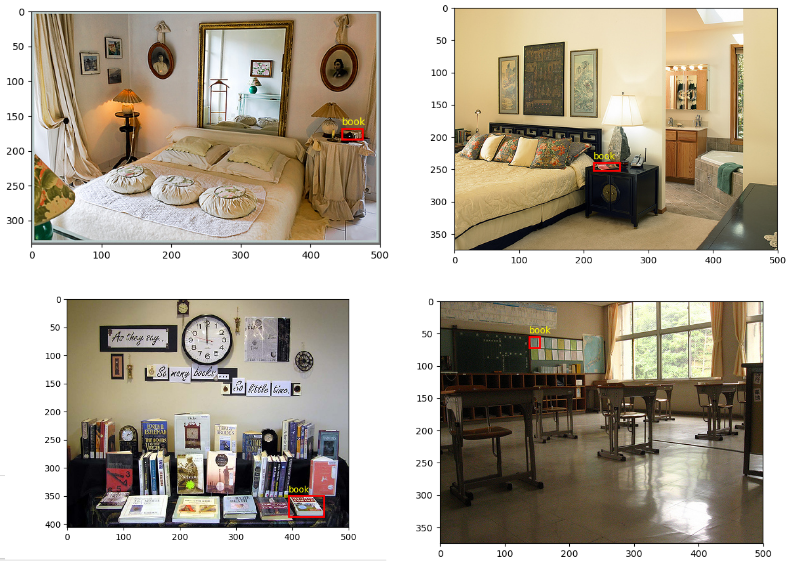
\includegraphics[width=1.0\hsize]{./figures/bookDifficult}
	\caption{The difficulties of detecting books in our ImageNet dataset: the books are really small inside the image (images at higher layer) and sometimes the annotation is either partial (bottom-left image) or incorrect (bottom-right image).}
	\label{fig:bookDifficult}
\end{figure}

\begin{figure}[tb]
	\centering
	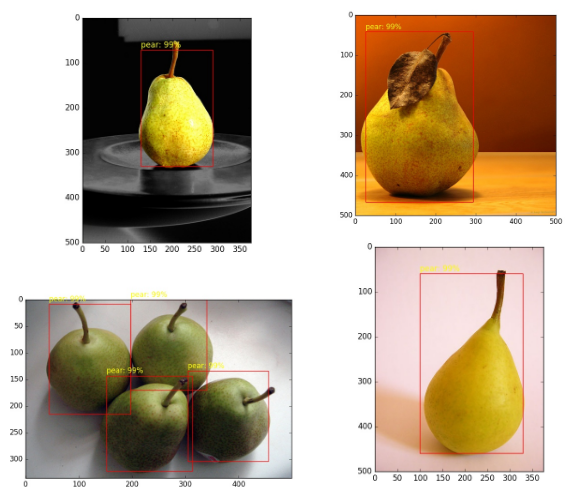
\includegraphics[width=1.0\hsize]{./figures/pear}
	\caption{The class \tit{pear} has small dataset too, however, images belong to this class are clearer and easier. We can see very accurate predictions in the four test images above.}
	\label{fig:pear}
\end{figure}

\begin{figure}[tb]
	\centering
	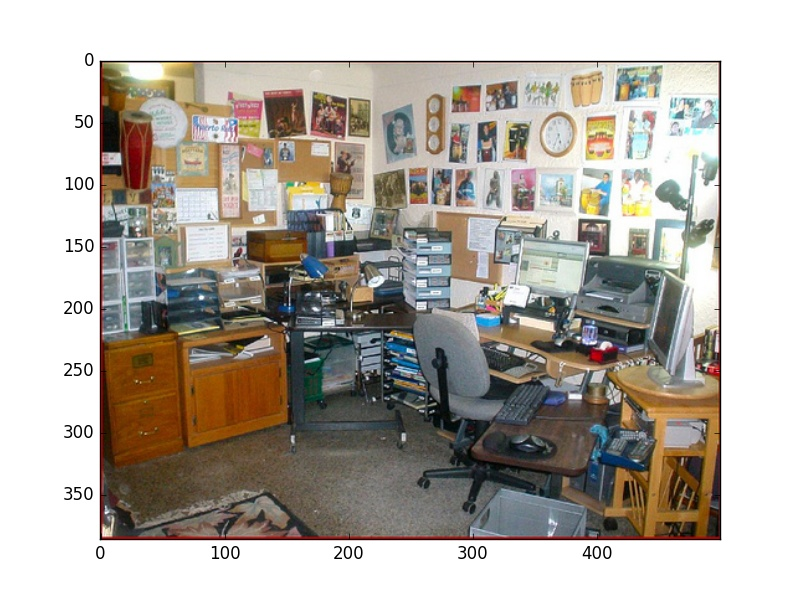
\includegraphics[width=0.8\hsize]{./figures/messyOffice}
	\caption{The objects in 3 classes \tit{monitor}, \tit{mouse}, \tit{pen} often go together in the office place. However, there are offices with a lot of objects.}
	\label{fig:messyOffice}
\end{figure}

\begin{figure}[tb]
	\centering
	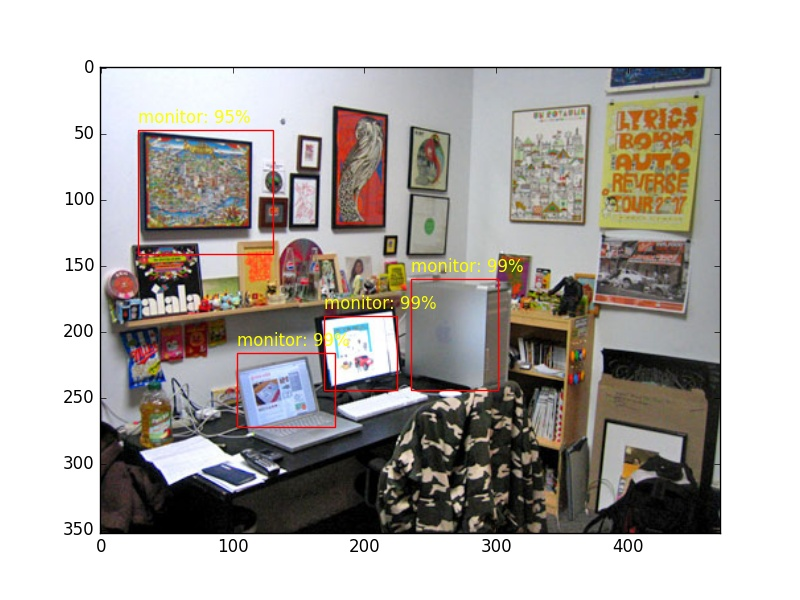
\includegraphics[width=0.8\hsize]{./figures/similarObj}
	\caption{False Positive due to object similarity: wall photo vs monitor.}
	\label{fig:similarObj}
\end{figure}

\begin{figure}[tb]
	\centering
	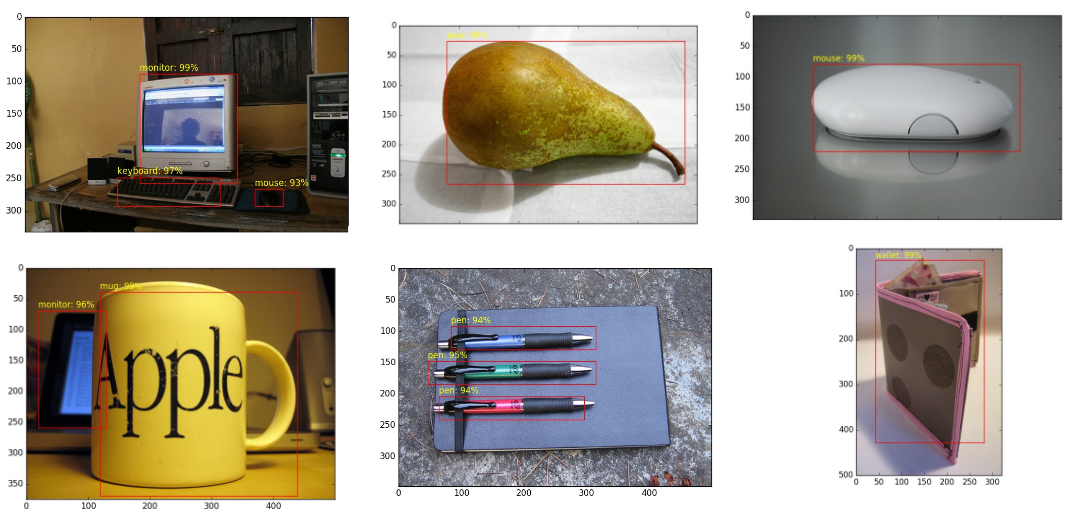
\includegraphics[width=1.0\hsize]{./figures/objDetImgNet}
	\caption{Object Detection with ImageNet: Run our Object Detection System on images in testset from our ImageNet dataset.}
	\label{fig:objDetImgNet}
\end{figure}

\begin{figure}[tb]
	\centering
	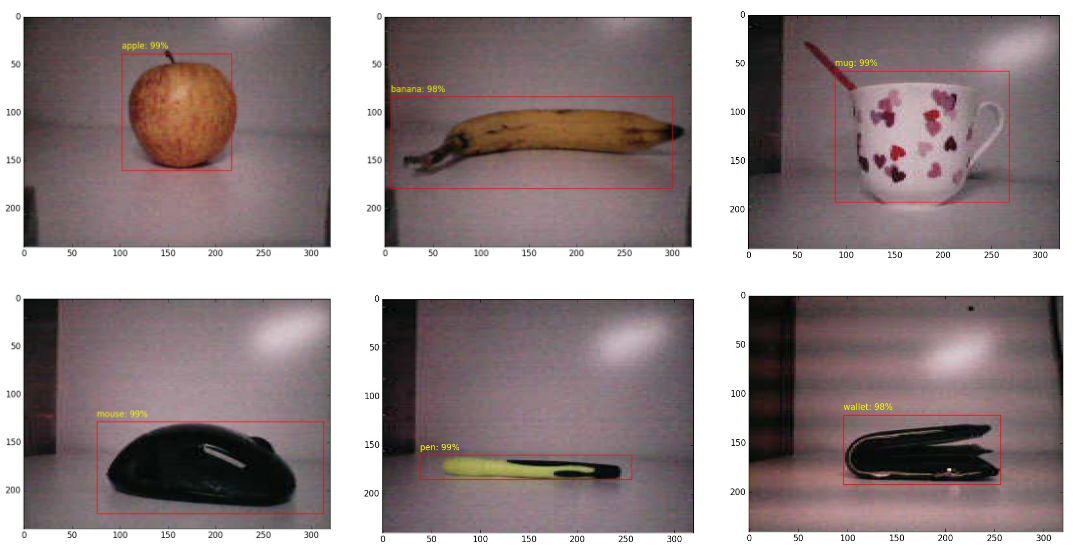
\includegraphics[width=1.0\hsize]{./figures/objDetCozmo}
	\caption{Object Detection with Cozmo's images: Run our Object Detection System on photos taken by Cozmo's camera.}
	\label{fig:objDetCozmom}
\end{figure}

\begin{figure}[tb]
	\centering
	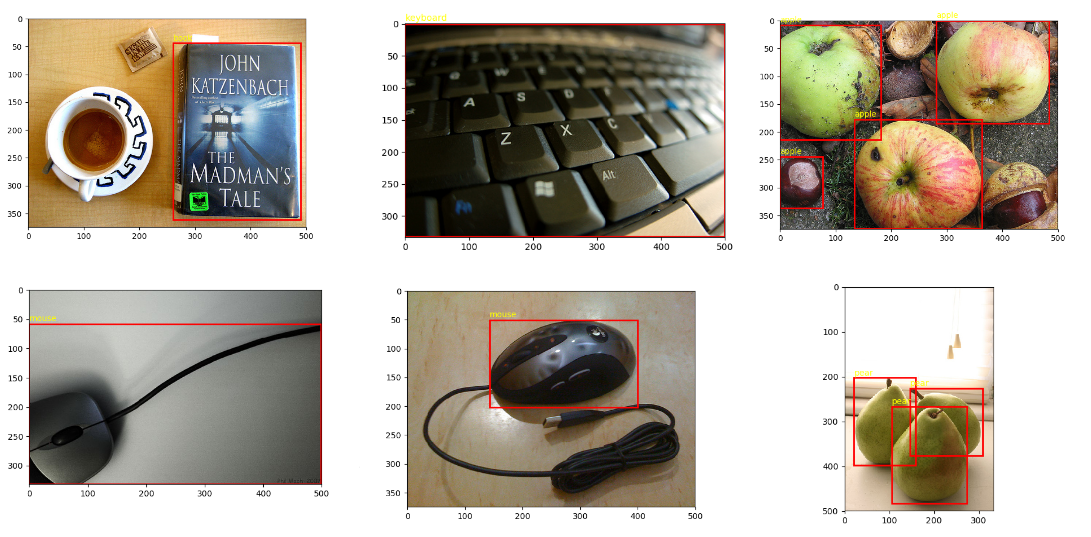
\includegraphics[width=1.0\hsize]{./figures/generalDifficult}
	\caption{Some limitations of ImageNet dataset: partial, inconsistent and incorrect annotation, "fullscreen" and overlapping objects.}
	\label{fig:generalDifficult}
\end{figure}


